\section{Detalles de la implementaci\'on}

En esta secci\'on se va a tratar de aclarar algunos puntos de la implementaci\'on del software, como el diagrama de clases y las optimizaciones de c\'odigo para reducir el tiempo de ejecuci\'on.\\

El c\'odigo completo realizado para este proyecto no se puede mostrar aqu\'i por motivos de espacio. Se aporta como anexo. Para ejecutar el programa basta con invocar el script \textit{genetreec.py} con python. El script dar\'a error si no se han instalado los paquetes necesarios (véase secci\'on \ref{sec:install}).\\

Todo el c\'odigo se encuentra comentado con las aclaraciones que se han cre\'ido necesarias.\\


El software se divide en cuatro archivos:\\

\begin{itemize}
    \item \textbf{genetreec.py}. Es el n\'ucleo del programa. Contiene las clases \textit{Simulate}, \textit{TreeStrategy} y \textit{EndStats}, necesarias para simular el \textit{backtesting}. Tiene una fuerte dependencia con el paquete \textit{backtrader}.
    
    \item \textbf{indicator.py}. Posee todos los indicadores usados y la herramienta para llamarlos y evaluar las fechas que se requiera.
    
    \item \textbf{tagger.py}. Etiqueta los datos para el calentamiento. 
    
    \item \textbf{tree.py}. En \'el est\'a la definici\'on de \'arbol, as\'i como las hojas y los nodos. Contiene las clases \textit{Leaf}, \textit{Node} y \textit{Tree}
\end{itemize}

\subsection{Diagrama de clases}

     	\begin{figure}[H]
    		\centering\leftskip=-100px
    		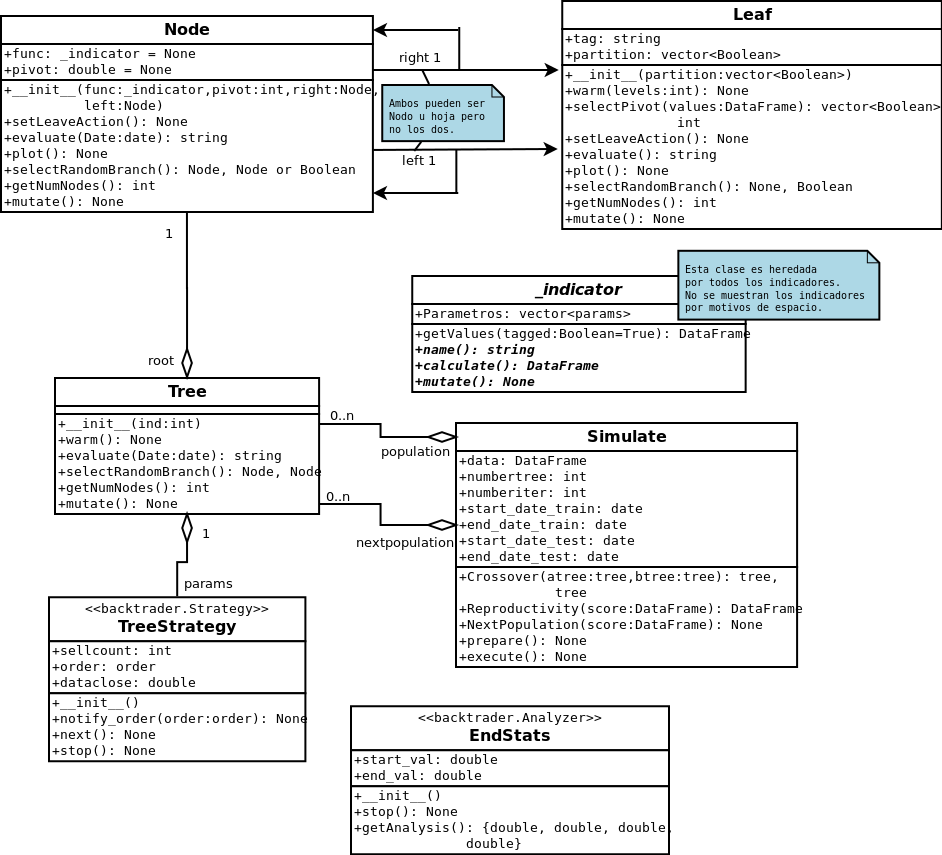
\includegraphics[scale=0.60]{imagenes/diagramaClases.png}
    	    \caption[Diagrama de clases del software desarrollado.]{Diagrama de clases del software desarrollado.\\ Fuente: elaboraci\'on propia}
    		\label{fig:diagclases}
	   \end{figure}

\subsection{Optimizaciones}\label{sec:timeimprove}

Los algoritmos evolutivos suelen tener unos buenos resultados, no solo por su caracter natural, si no por su amplia capacidad para inspeccionar el espacio de b\'usqueda cercano a las buenas soluciones.\\

En espacios de b\'usqueda amplios, como es el caso, las combinaciones son muy grandes y las b\'usquedas se alargan mucho. A esto hay que a\~nadirle el peso de la funci\'on \textit{fitness} que, en este caso, conlleva simular un periodo de bolsa y evaluar muchas veces los indicadores en distintas fechas. Adem\'as, se dispone de una m\'aquina bastante modesta para su ejecuci\'on.\\

Todos estos inconvenientes hacen necesario poner especial cuidado a la hora de realizar el software e intentar reducir el gasto tanto de tiempo como de espacio. Si bien este \'ultimo, en principio, no nos producir\'a problema.\\

\subsubsection{Paralelizaci\'on}
Al utilizar \textit{backtrader} en la introducci\'on (v\'ease \ref{sec:backtrader}) se mostraron varios ejemplos sencillos de uso. Pero el paquete dispone de otras opciones que permiten adaptarlo a nuestras necesidades. Se comentar\'a, a continuaci\'on, la posibilidad de ejecutar en paralelo.\\

Lo primero que se debe reformular para poder ejecutar en paralelo es la estrategia. Como se concret\'o, la clase \textit{cerebro} recibe una estrategia como par\'ametro, que es quien da las se\~nales de compra y venta. De esta forma, si se simulase cada uno de los \'arboles de la poblaci\'on, digamos 50, se tendr\'ian que crear 50 cerebros, a\~nadir 50 veces los datos y simular 50 veces las mismas fechas (cada vez con un individuo distinto).\\

Para corregir este comportamiento, se sugiere usar la funci\'on \textit{optstrategy} de la clase \textit{cerebro} de la siguiente forma:\\

\begin{lstlisting}
cerebro.optstrategy(TreeStrategy,tree=list(population))
\end{lstlisting}

En realidad, esta funci\'on est\'a pensada para a\~nadir una rejilla de par\'ametros que matizan la estrategia definida. En lugar de esto, nosotros vamos a pasar la propia poblaci\'on de \'arboles como rejilla de par\'ametros.\\

Una vez realizado este cambio, \textit{backtrader} ejecutar\'a la estrategia con los distintos \'arboles de forma iterativa. No es necesario cargar los datos m\'ultiples veces, basta con una sola copia de estos.\\

Ahora vamos a eliminar la linealidad de ejecuci\'on. \textit{backtrader} permite ejecutar de forma paralela una estrategia a la que se ha aportado una rejilla de par\'ametros. Con la directiva \textit{cerebro = bt.Cerebro(maxcpus=None)} indicamos que no hay l\'imite de n\'ucleos para la ejecuci\'on. \\

La m\'aquina usada dispone de 4 n\'ucleos. Esto nos da una mejora signficativa de tiempo, ya que nos permite evaluar 4 individuos a la vez. Cuantos m\'as n\'ucleos tenga la m\'aquina, m\'as acentuada ser\'a la mejora.\\


\subsubsection{Cach\'e para indicadores de primer orden}
La parte computacional m\'as costosa es la evaluaci\'on de los indicadores. El c\'alculo de algunos de ellos depende de los valores de la acci\'on de varios d\'ias atr\'as. Cargar esos datos y hacer las operaciones repetidas veces es un gasto innecesario de tiempo.\\

Adem\'as los \'arboles tienen varios niveles de profundidad. Para cada d\'ia que se simule la inversi\'on, se calculan la misma cantidad de indicadores que de niveles.\\

En un intento de reducir esto, se va usar el paquete de \textit{Python} \textit{TA-Lib}\footnote{\url{https://mrjbq7.github.io/ta-lib/doc_index.html}. \'Ultima consulta 25 de Julio de 2019}.
\textit{TA-Lib} es un paquete de c\'alculo para indicadores t\'ecnicos de bolsa. Este software est\'a pensado para calcular un gran n\'umero de indicadores de bolsa a lo largo de un periodo, es decir, aportados los valores de un periodo de tiempo, te devuelve el indicador en el mismo periodo.\\

Un caso de uso ser\'ia el siguiente, en el que se calcula el indicador \textit{EMA}:\\

\begin{lstlisting}
data['EMA'] = talib.EMA(df['Close'], period)
\end{lstlisting}

La fuerza de este paquete reside en la capacidad de calcular indicadores en espacios de tiempo grande. Para sacar partido de este hecho, en lugar de ir calculando los indicadores en los d\'ias que nos interesan, se va a optar por calcularlo en todos los d\'ias del periodo.\\

Se realiza entonces un \textit{DataFrame} en el que se van almacenando todos los indicadores calculados. Cada vez que se quiere acceder a un indicador en una fecha, primero se comprueba si est\'a ya calculado y, en caso negativo, se calcula y se guarda. Este almac\'en puede perdurar incluso entre distintas generaciones, ya que los \'arboles deber\'ian tener indicadores con par\'ametros iguales en muchos casos.\\ 

De forma sistem\'atica, cuando se requiera un indicador, se acceder\'a a la funci\'on \textit{getValues} de cada indicador, que mantiene esta estructura de guardado de datos:\\

\begin{lstlisting}
def getValues(self):
	if self.name() in df.columns.values:  # df es global
		return df[self.name()]
	else:
		return self.calculate()
\end{lstlisting}

Para guardar los datos, cada columna se ha nombrado de forma \'unica para cada indicador. El nombre se conforma por el nombre del indicador y los par\'ametros que hubiere.\\

\subsubsection{Cach\'e para indicadores de segundo orden}

La primera cach\'e elimina coste computacional calculando los indicadores en todas las fechas de una sola vez. Ahora surge un problema provocado por este hecho, cada d\'ia hay que acceder a los indicadores de ese d\'ia en unas 4 o 5 ocasiones (una por nivel de profundidad).\\

Por consiguiente, se van a producir en la simulaci\'on del mismo d\'ia varias b\'usquedas en un \textit{DataFrame} cuyo \'indice son fechas. A priori, se podr\'ia pensar que buscar por fechas es igual que buscar por un entero, pero no es as\'i. \textit{Python} tiene un tipo especial para tratar con fechas que hace que las b\'usquedas se ralenticen mucho.\\

Para evitar esta coste adicional de b\'usqueda, se propone realizar un segundo nivel de cach\'e. En esta ocasi\'on, este almac\'en va a guardar los indicadores del \'ultimo d\'ia del que se pidi\'o un indicador. \\

Como en el mismo d\'ia se va a requerir el uso de varios indicadores, estamos ahorrando b\'usquedas en el \textit{DataFrame} que conforma la primera cach\'e.\\

     	\begin{figure}[H]
    		\centering\leftskip=-30px
    		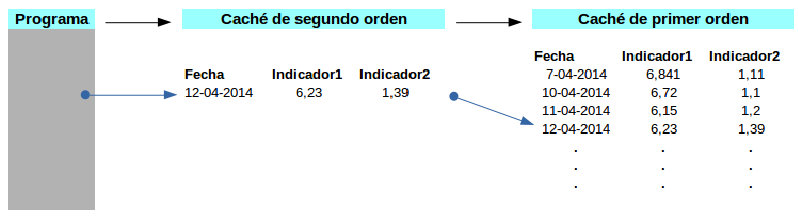
\includegraphics[scale=0.60]{imagenes/caches.png}
    	    \caption[Estructura de las cach\'es]{Estructua de las cach\'es.\\ Fuente: elaboraci\'on propia}
    		\label{fig:caches}
	   \end{figure}
	   
El c\'odigo sigue la misma idea que el desarrollado para la primera cach\'e, solo hay que tener en cuenta que es necesario hacer una nueva variable global para guardar los datos del d\'ia. Adem\'as, ahora la cach\'e puede fallar por dos motivos distintos. El primero que el indicador no est\'e en la primer cach\'e, por tanto es necesario calcular los valores del indicador e incluirlos en el \textit{DataFrame}. Y el segundo, que los datos guardados en la segunda cach\'e sean de otro d\'ia, en cuyo caso es necesario cargar el d\'ia correcto en \'esta.\\

\begin{lstlisting}
def getValueByIndex(index, func):
	global thisday
	if func.name() in thisday.columns.values:
		if thisday.index != index:
			thisday = df.loc[[index]]
		return thisday[func.name()][0]
	ret = func.getValues(False).loc[index]
	thisday = df.loc[[index]]
	return thisday[func.name()][0]
\end{lstlisting}
